% !TEX root = main.tex

% TODO:
% REMARK:
% . * Don't mention LHC, CMS, etc. in this section, just have a historical review ana provide physical motivation to the study

\section{Introduction}
\label{sec:Introduction}

	The violation in combination of charge conjugation(C) and parity(P) is called $\textbf{CP}$ $\textbf{violation}$$\textbf{(CPV)}$. It has been alredy investigate in physics like $K_L$-meson decay. In the modern standard model(SM), the CP violation appears in CKM(Cabibbo– Kobayashi–Maskawa) matrix which consists of mixing(rotation) angle of three generation quarks weak interaction. CPV is actually introduced from irreducible complex phase in CKM matrix as quark sectors. We could easily see it in the wildy used Wolfenstein parameterisation with CKM matrix:

	\begin{equation}
  		\begin{pmatrix}
  		V_{ud} & V_{us} & V_{ub} \\
  		V_{cd} & V_{cs} & V_{cb} \\
  		V_{td} & V_{ts} & V_{tb} \\
  		\end{pmatrix}
  		=
  		\begin{pmatrix}
  		1 - \lambda^2/2 & \lambda & A \lambda^3(\rho -i \eta) \\
  		-\lambda & 1 - \lambda^2/2 & A \lambda^2 \\
  		A \lambda^3(1 - \rho -i \eta) & - A \lambda^2 & 1 \\
  		\end{pmatrix} 
  		+ O(\lambda^4)
	\end{equation}

	Investigation and experiments to strange/bottom sectors are already researched. However, all the known CPV source including quarks sector are not sufficient to explain the observed matter-antimatter asymmetry in the universe. The CP violation in SM $t\bar{t}$ is predicted very small as presenting in LHC. Nevertheless, with the LHC being a top quarks factory, if there is possible model being source of CPV like CEDM, 2HDM, MSSM..., there would be evident signal. That is, with big cross section of $t\bar{t}$, the measurement of asymmetry in $t\bar{t}$ would be a valuable probe for matter-antimatter asymmetry.(ref.\cite{Olive_2014})

	\subsection{CP Violation in $t\bar{t}$ and possible sources}
	\label{ssec:Intro_CPVpossible}

		The possible source, which is also the primary focus in this analysis, of the CPV in $t\bar{t}$ is the anomalous top quark coupling affecting both decay and production of $t\bar{t}$. The anomalous coupling in $t\bar{t}$ production might be induced by the $\textbf{chromo}$ $\textbf{electric}$ $\textbf{dipole moment(CEDM)}$ of the interaction with top quark. The original CEDM lagragian density is coupled with $\textbf{chromo}$ $\textbf{magnectic}$ $\textbf{dipole}$ $\textbf{moment(CMDM)}$ defined as:

		% original L
		\begin{equation}
		\begin{split}
		L_{cdm} = \frac{g_s}{2} \bar{t} T^a\sigma^{\mu \nu}(a_t^g + i \gamma^5 d_t^g) t G^a_{\mu \nu}
		\label{eq:CEDM_L_ori}
		\end{split}
		\end{equation}
		\FloatBarrier

		The $d_t^g$ and $a_t^g$ in Eq.\ref{eq:CEDM_L_ori} are top CEDM and CMDM parameters; The $G^a_{\mu \nu}$ is the gluon field strength interacting with top quarks; the $\sigma^{\mu \nu}$=$(i/2) [\gamma^{\mu},\gamma^{nu}]$.
		The $d_t^g$ in the lagragian is the CP-odd CEDM parameter with both real part $Re(d_t^g)$ and imaginary part $Im(d_t^g)$. \cite{Zhou:1998wz} The real part of $d_t^g$ is referred to the dipersive part and the imaginary part of $d_t^g$ is also regarded as absorptive part. In the production part, the top CEDM $d_t^g$ contributes to the CP violating amplitudes with the Feynman diagram depicted in Fig.\ref{Intro:fig:qqgg_tt}.

		% qq->tt, gg->tt diagram
		\begin{figure}[H]
		\centering
			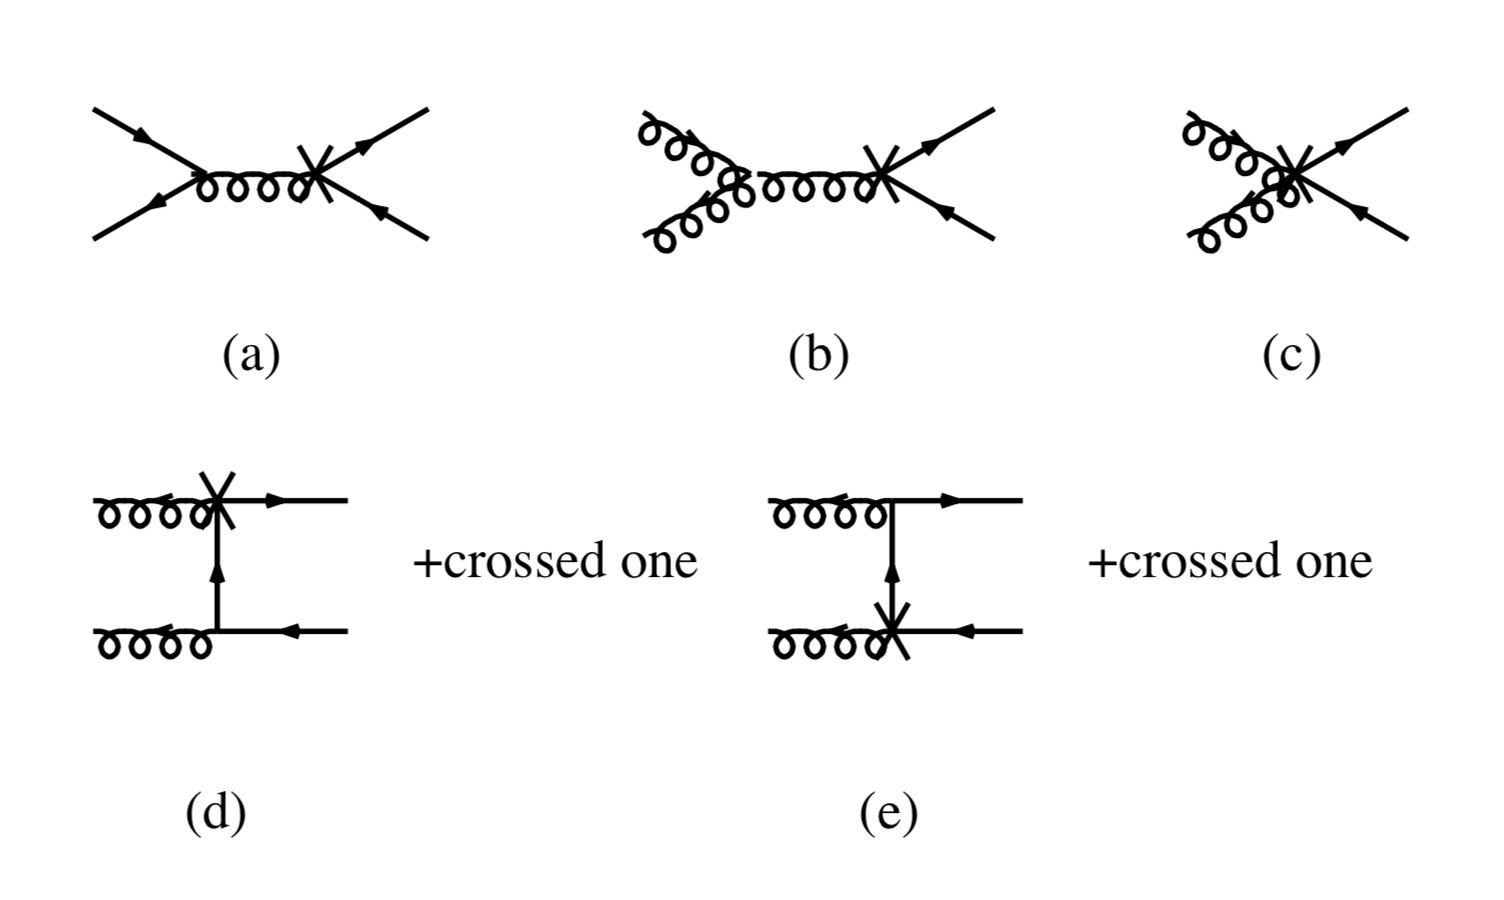
\includegraphics[width=0.85\textwidth]{Figures/Intro/qqgg_tt.png}
		\caption{Tree level Feynman diagram for $qq \rightarrow t\bar{t}$ and $gg \rightarrow t\bar{t}$, the crosses in diagrams denote the vertices modified by top CEDM \cite{Zhou:1998wz}}
		\label{Intro:fig:qqgg_tt}
		\end{figure}
		\FloatBarrier

		After the Higgs boson's discovered and standard model's development, Eq.\ref{eq:CEDM_L_ori} is not appropriate to the gauge invariance and symmetry of standard model. That is to say, any new physics must come in the form of an effective Lagrangian that respects all the symmetries of the SM, in particular the SU(2)(weak interaction) symmetry. This symmetry forbids couplings in Eq.\ref{eq:CEDM_L_ori}. The form of lagrangian in Eq.\ref{eq:CEDM_L_ori} could be reserve but to adapt it, the correct gauge invariant, operators must include a Higgs field. The adaptive form is shown in Eq.\ref{eq:CEDM_L_ada}.

		% adapted L after SM
		\begin{equation}
		\begin{split}
		L_{cdm} = g_s \frac{d_{tG}}{\Lambda^2} \bar{q_3} T^a\sigma^{\mu \nu} t \widetilde{\phi} G^a_{\mu \nu} + H.c.
		\label{eq:CEDM_L_ada}
		\end{split}
		\end{equation}
		\FloatBarrier

		where the $q_3$ is the third generation SM quark doublet, $\widetilde{\phi}$ is the scalar doublet, and the $T^a$ are the SU(3) generators. The relation between $d_{tG}$ and $d_t^g$ is shown(Eq.\ref{eq:CEDM_L_connection}). then the absorptive part of form factor $d_t^g$ which arises from a loop should not be written down in lagrangian.

		\begin{equation}
		\begin{split}
		d_t^g = \frac{\sqrt{2} v}{\Lambda^2} Im(d_{tG})
		\label{eq:CEDM_L_connection}
		\end{split}
		\end{equation}
		\FloatBarrier

		In addition to the CPV from CEDM in production of $t\bar{t}$, there are also CP violation, which is the anomalous coupling $f$, arise in the vertices of $t\bar{t}$ with the decay $t \rightarrow bW^+$ and $\bar{t} \rightarrow \bar{b}W^-$, and would arise in the vertices of $t\bar{t}$. The $f$ is composed of CP conserving phase $\delta_f$ and CP violating phase $\phi_{f}$ with $\widetilde{f}$ parametrised. The vertices are shown below Eq.\ref{eq:CEDM_CPV_decay}, ref.\cite{PhysRevD.81.034013}:

		\begin{equation}
		\begin{split}
		\Gamma^{\mu}_{W_{tb}} = - \frac{g}{\sqrt{2}}V_{tb}^{*} \bar{u}(p_{b})[ \gamma_{\mu} P_{L} - i\widetilde{f}e^{i(\phi_f + \delta_f)} \sigma^{\mu \nu} (p_t - p_b)_{\nu} P_R ] u(p_t) \\
		\bar{\Gamma}^{\mu}_{W_{tb}} = - \frac{g}{\sqrt{2}}V_{tb} \bar{v}(p_{\bar{t}})[ \gamma_{\mu} P_{L} - i\widetilde{f}e^{i(-\phi_f + \delta_f)} \sigma^{\mu \nu} (p_{\bar{t}} - p_{\bar{b}})_{\nu} P_L ] v(p_{\bar{b}})
		\end{split}
		\label{eq:CEDM_CPV_decay}
		\end{equation}
		\FloatBarrier

		These two CP violating anomalous couplings, $d_t^g$ and $\widetilde{f} \sin{\phi_f}$, have induced the T-odd correlation, so it is considered to use T-odd observables.(ref.\cite{PhysRevD.81.034013},\cite{PhysRevD.79.013013},\cite{PhysRevD.80.034013}) Besides, there are some probable models could be the source of CP violation in $t\bar{t}$ like 2HDM model. There are some discussion in section.\ref{sssec:AcpModel_2HDM} The emphasis of this analysis is to focus on approach to the top CEDM phenomenon.

		% mainly to detect CEDM, theory part of CEDM

	\subsection{Triple product observables to detect CP violation in LHC}
	\label{ssec:Intro_TPinLHC}

		% intro of naive T, T-odd, T-even. focus on T-odd
		% used 4 observables, why? corresponding to detector

		To approach the possibility of CP violation in sample, the time reversal would be introduced because of the assumption of CPT conservation, which indicates that all the physical states are the eigenstates of CPT operator in the universe. Therrefore, the observables we used in the analysis are the triple product observables which are exactly $\textbf{T-odd}$ $\textbf{observables}$. The $T$ here means the time reversal operator, more accurately, this is the $\textbf{naive}$ $\textbf{time}$ $\textbf{reversal}$ $\textbf{operator}$ $\textbf{T}_N$. The ordinary time reversal operator means that it changes signs of the momenta and spins of all particles and also exchange the initial and final states. The naive time operator, however, is the time reversal without interchanging between initial state and final state. The advantage of naive time reversal is that the initial state's detection and calculations are not available for usual decay process in experiment. That is to say, if the combination of charge and parity is not conserved, the kinematics of final state would tell the CP-violation story. The applied observable -- T-odd triple product observables, which basic form is shown below(Eq.\ref{eq:triple_product_form}):(ref.\cite{PhysRevLett.58.451},\cite{PhysRevD.80.034013})

		\begin{equation}
		O = \vec{v_{1}} \cdot ( \vec{v_2} \times \vec{v_{3}} )
		\label{eq:triple_product_form}
		\end{equation}
		\FloatBarrier

		where the $v_{1,2,3}$ are the momentum or spins vectors. It is obvious to be T-odd($T_{N}$-odd) type because there are three components. Furthermore, there are also some T-even observables but not the usage of this analysis. Also, the combinations of these three vectors would be CP-odd or CP-even type of triple product. The CP-odd(CP-even) means the eigenvalue of CP eigenstate is -1(+1). The prefered triple product observables are commonly the CP-odd observables, take the observable $O = \vec{p_{l^-}} \cdot ( \vec{p_{t}} \times \vec{p_{\bar{t}}} )$ in \cite{PhysRevLett.58.451} for example:

		\begin{equation}
		\begin{split}
		p_{t}\xrightarrow[\text{}]{\text{CP}} -p_{\bar{t}} \; \; , \; \; p_{t}\xrightarrow[\text{}]{\text{CP}} -p_{\bar{t}} \; , \; \; \\
		p_{l^-} \xrightarrow[\text{}]{\text{CP}} p_{l^-} \; \; , \; \; p_{l^-} \xrightarrow[\text{}]{\text{CP}} p_{l^+} \;, \\
		\vec{p_{l^-}} \cdot ( \vec{p_{t}} \times \vec{p_{\overline{t}}} ) \xrightarrow[]{\text{CP}} \vec{p_{l^-}} \cdot ( - \vec{p_{\overline{t}}} \times - \vec{p_{t}} ) \\
		= \vec{p_{l^-}} \cdot ( \vec{p_{t}} \times \vec{p_{\overline{t}}} ) \;\;\;\;\;\;
		\end{split}
		\label{eq:ex_obs_eett}
		\end{equation}
		\FloatBarrier

		where the CP-odd property is trivially acting lile the formula above. In the analysis, we only put emphasis on the CP-odd observables. Given a CP-odd observable, we can define an asymmetry measurement in Eq.\ref{eq:asymmetry_form} which is established on counting events between positive and negative value of observable. The $O_i$ in Eq.\ref{eq:asymmetry_form} means the CP-odd observables and different observables have different sensitivity to the CP violation if there is new physics involved.

		\begin{equation}
		A_{cp} = \frac{ N_{events}(O_i>0) - N_{events}(O_i<0) }{ N_{events}(O_i>0) + N_{events}(O_i<0) }
		\label{eq:asymmetry_form}
		\end{equation}
		\FloatBarrier

		% development of triple product observable
		Under the form Eq.\ref{eq:triple_product_form} and the CP-odd design Eq.\ref{eq:asymmetry_form}, we can easily build T-odd observables for detecting CP violation. \\
		
		To discuss about the general case of T-odd triple product observable, there is a simple case -- the $\textbf{inclusive case}$, which is the jets' information used only. The parity operator would change the sign of four momentum, but the charge conjugate could not change the jets' sign because it is summed over by particles and antiparticles in defining the jets. There are 3 jets' momenta ordered by energy or spread by $p_{\perp}$($E_1$>$E_2$>$E_3$ or $p_{\perp 1}$ > $p_{\perp 2}$ > $p_{\perp 3}$). They are also used to form a CP-odd triple product $J$(Eq.\ref{eq:inclusive_obs1}, ref.\cite{PhysRevLett.58.451}):

		\begin{equation}
		J = \vec{p}_1 \cdot \vec{p}_2 \times \vec{p}_3
		\label{eq:inclusive_obs1}
		\end{equation}
		\FloatBarrier

		however, there is a adapted one with beam direction $\vec{p}$ and some total polarization $\vec{S}$ perpendicular to the beam direction. They both are unchanged under CP operation, so the rest one is dropped a jet four momentum to make it CP-odd still. The form is shown in Eq.\ref{eq:inclusive_obs2}(ref.\cite{PhysRevLett.58.451}.

		\begin{equation}
		\widetilde{J} = \vec{p}_- \times \vec{S} \cdot \vec{p}_{jet}
		\label{eq:inclusive_obs2}
		\end{equation}
		\FloatBarrier

		Another case is the $\textbf{semi-inclusive case}$. When the particles identification is improved, the particles is not merely labeled by its four momentum. Therefore, there are wider tests could be adopted to do CP-test, and it is exactly more effective in the modern collider experiments. We denote the flavor of particles as $F$ and their anti-particles as $\bar{F}$, the possible observable terms are shown(Eq.\ref{eq:semi_inclusive_obs},ref.\cite{PhysRevLett.58.451}):

		\begin{equation}
		\begin{split}
		\vec{p}_- \times \vec{p}_{jet} \cdot ( \vec{p}_F - \vec{p}_{\bar{F}} ) \;\;, \;\; \vec{S} \times \vec{p}_{jet} \cdot ( \vec{p}_F - \vec{p}_{\bar{F}} ) \\
		\vec{p}_- \times \vec{S} \cdot ( \vec{p}_F + \vec{p}_{\bar{F}} ) \;\;, \;\; \vec{p}_{jet,1} \times \vec{p}_{jet,2} \cdot ( \vec{p}_F + \vec{p}_{\bar{F}} ) \\
		\vec{p}_- \cdot ( \vec{p}_F \times \vec{p}_{\bar{F}} ) \;\;,\;\; \vec{S} \cdot ( \vec{p}_F \times \vec{p}_{\bar{F}} )
		\label{eq:semi_inclusive_obs}
		\end{split}
		\end{equation}
		\FloatBarrier

		The $(\vec{p}_F + \vec{p}_{\bar{F}})$ in Eq.\ref{eq:semi_inclusive_obs} means the particle and anti-particle are not necessary to be really distinguished, for example, it is acceptible that the charges of 2 same flavor jets are not clearly assigned under the type of observable. On the other hand, the $(\vec{p}_F - \vec{p}_{\bar{F}})$ and $(\vec{p}_F \times \vec{p}_{\bar{F}})$ need more accuracy at seperating particle and anti-particle. Moreover, there is also a CP-odd type but T-even observables like Eq.\ref{eq:3vec_Teven}, but it is not used in this real data analysis. T-even observables will be discussed more in section.\ref{ssec:AcpObs}.

		\begin{equation}
		\vec{p}_{jet} \cdot ( \vec{p}_F - \vec{p}_{\bar{F}} )
		\label{eq:3vec_Teven}
		\end{equation}
		\FloatBarrier

		% related to this analysis

		For the LHC experiment, the proton-proton initial state is not a CP eigenstate. Also, under the LHC's energies, the dominant gluon fusion initial state($gg \rightarrow t\bar{t}$) is not CP eigen state, either. However, summing over gluon's flavors and colors could achieve CP-odd observables which in the similar way as the jets observables. There are three channel for $t\bar{t}$ decay -- hadronic channel, leptonic channel, and single lepton+jets channel. The hadronic channel presents both of W bosons decay to two jets respectively, and the leptonic channel assumes both of W boson decay to lepton and neutrino which is detected as Missing $E_T$ in analysis. The analysis is to probe CP violation in $t\bar{t}$ semileptonic decay Eq.\ref{eq:semileptonic_decay}, where both top quarks decay to bottom quarks and W bosons. Then one of W bosons decays and ends up with being recognized as 2 jets($j_1$,$j_2$), and the other one decays to lepton and neutrino. All of suitable observables for each channel are researched in ref.\cite{PhysRevD.80.034013},\cite{PhysRevD.81.034013},\cite{Hayreter:2015ryk}.

		\begin{equation}
		t\bar{t} \rightarrow b\bar{b} W^+W^- \rightarrow b\bar{b} jj l \nu
		\label{eq:semileptonic_decay}
		\end{equation}
		\FloatBarrier

		There are more organized T-odd triple product observables in ref.\cite{Hayreter:2015ryk} for leptonic channel and single lepton+jets channel. Yet, there are some constraint to make it valid in real experiments. For instance, the $O_1$ in\cite{Hayreter:2015ryk} is $\epsilon(p_t,p_{\bar{t}},p_b,p_{\bar{b}}) = \epsilon_{\mu \nu \rho \zeta}p_t^{\mu}p_{\bar{t}}^{\nu}p_b^{\rho}p_{\bar{b}}^{\zeta} \xrightarrow[]{t\overline{t}CM} \vec{p_t} \cdot ( \vec{p_b} \times \vec{p_{\overline{b}}} )$, where the $\epsilon$ is the Levi–Civita tensor and $p_i^{\alpha}$ is the four momentum of i particle. The $p_t$ in $O_1$ have to be reconstructed with information from detector, and the neutrino's z-direction's(collided beam's direction) information could be missed in detector.

		According to the final states' resolution and reconstruction, there are four appropriate observables:

		\begin{equation}
		\begin{split}
		O_3 = Q_l \epsilon(p_{b}, p_{\bar{b}}, p_{l}, p_{j_1}) \xrightarrow[\text{}]{b \bar{b} CM} Q_l \vec{p_{b}} \cdot ( \vec{p_l} \times \vec{p_{j_1}} ) \\
		O_{6} = Q_l \epsilon(P, p_{b}-p_{\bar{b}}, p_{l}, p_{j_1}) \xrightarrow[\text{}]{lab} Q_l (\vec{p_{b}} - \vec{p_{\overline{b}}}) \cdot ( \vec{p_l} \times \vec{p_{j_1}} ) \\
		O_{12} = q \cdot (p_{b}-p_{\bar{b}}) \epsilon(P_{}, q, p_{b}, p_{\bar{b}}) \xrightarrow[]{lab} (\vec{p_{b}} - \vec{p_{\overline{b}}})_z ( \vec{p_b} \times \vec{p_{\overline{b}}} )_z \\
		O_{14} = \epsilon(P, p_{b}+p_{\bar{b}}, p_{l}, p_{j_1}) \xrightarrow[]{lab} (\vec{p_{b}} + \vec{p_{\overline{b}}}) \cdot ( \vec{p_l} \times \vec{p_{j_1}} )
		\end{split}
		\label{eq:four_obs}
		\end{equation}
		\FloatBarrier

		The $j_1$ is the leading $p_T$ jets except the chosen b-flavor jets; $l$ refers to muon or electron, and $Q_l$ is the electric charge of lepton $l$; Also, the $\rightarrow$ and the text above indicates the spacetime frame chose to observe the properties. All the four observables are confirmed CP-odd and available in counting events asymmetry(Eq.\ref{eq:asymmetry_form}). 

		\begin{equation}
		\begin{split}
		\vec{p}_b \overset{CP}{\longleftrightarrow} -\vec{p}_{\overline{b}}\;\;, \;\; \vec{p}_{l^-} \overset{CP}{\longleftrightarrow} -\vec{p}_{l^+}\;\;,\;\;\;\;\;\; \\
		\vec{p}_{j_1} \overset{CP}{\longleftrightarrow} -\vec{p}_{j_1}\;\;, \;\; Q_{l^+} \overset{CP}{\longleftrightarrow} -Q_{l^+} = Q_{l^-}
		\label{eq:CP_rule}
		\end{split}
		\end{equation}
		\FloatBarrier

		Following the CP operator's effect(Eq.\ref{eq:CP_rule}), take $O_6$ for example, the $\mu^+$ is from the case with $W^+$ is leptonic decay and $\mu^-$ is from the case with $W^-$ is leptonic decay(Eq.\ref{eq:O6ex}), it is exactly CP-odd:

		\begin{equation}
		\begin{split}
		O_6 = Q_l (\vec{p}_b - \vec{p}_{\bar{b}}) \cdot (\vec{p}_{\mu^-} \times \vec{p}_{j_1} + \vec{p}_{\mu^+} \times \vec{p}_{j_1}) \\
		\xrightarrow[]{CP} -Q_l (\vec{p}_{\bar{b}} - \vec{p}_b) \cdot (-\vec{p}_{\mu^+} \times \vec{p}_{j_1} + -\vec{p}_{\mu^-} \times \vec{p}_{j_1}) = -O_6
		\label{eq:O6ex}
		\end{split}
		\end{equation}
		\FloatBarrier

	\subsection{Experimental and data analysis strategy}
	\label{ssec:Intro_ExpDAStr}

		To really do the experiment to measure the CP violation in $t\bar{t}$, we use the dataset which is collected from $\textbf{Compact Muon Solenoid(CMS)}$ experiment in $\textbf{Large}$ $\textbf{Hadron}$ $\textbf{Collider(LHC)}$ under the institute $\textbf{European}$ $\textbf{Organisation}$ $\textbf{for}$ $\textbf{Nuclear}$ $\textbf{Research}$$\textbf{(CERN)}$. The simple concept of designing of CMS experiment's detector would be introduced in Chapter.\ref{sec:ExperimentalAppratus}. Moreover, the intermediate dealing with raw data to physical objectecs is necessary. The detail of physical objects reonstruction and the object selection will be shown in Chapter.\ref{sec:PhysObj}. As following, the analyzed data and simulation data will be represented in Chapter.\ref{sec:DataAndMC}. There are not only the real data taking shown, but also the simulated data's calibration and correction mentioned.

		It is the primary analysis part to extract the signal from all the messy data. Therefore, the Chapter.\ref{sec:EventSelReco} will tell the techniques to select the events and to reconstruct the confident fragment, and then to tell the probed part. In this analysis, we mainly compare the data and simulation with the invariant mass of top which decays hadronically to validate that our selected data is under a high confidence level of what we want. The objects kinematics and flavor information would be used to events selection, and the known top quark mass and W boson mass informations would be included to help distinguish the selected objects. In addition, the machine learning concept is added in the analysis to help discerning physical objects in final states. After selecting and reconstructing the events, the background, which means the events we have no interest on, should be ruled out although it stands less portion of all the events. The fitting skills would be adopted and the details are in Chapter.\ref{sec:BkgEst}. 

		The reconstruction and detector bias in the measurements play an critical roll because it is not quite direct to measure the physical object in CMS experiment. Chapter.\ref{sec:AsymBias} will discuss how the measurement affected by the reconstrruction and detector issue, also it will discuss how the observables react on the asymmetry measurement. The dilution effect from detector issue to calculation of $A_{cp}$ will discussed in Chapter.\ref{sec:Dilution}. Last but not least, there must be systematic uncertainty considered in any experiments. Chapter.\ref{sec:Systematic} demonstrate the systematic undertainty and their implementation.

		The baseline is mostly similar to the CMS run1's analysis(8TeV)\cite{Khachatryan:2016ngh}. There are some improvement of analysis input in the part of events selection and physical objects distinguishment with MVA tool. Therefore, one of the point we focus in this analysis is to compare the result of using original method($\chi^2_{min}$) and using new method(MVA) to distingusih the physical objects. Also, there are some research on the possible source(model) of CP violation in $t\bar{t}$, and the T-even observables' discussion are listed in the Chapter.\ref{sec:AcpModelObs}.

		The part of conclusion(Chapter.\ref{sec:Result}) collects the results in any chapters and organizes to be final results. There are comparison of method, precision of measurement, and the explanation of the demonstrated informations.


\FloatBarrier
